% Standalone TikZ for Figure 1: System Architecture (clean, high color, no overlap)
\documentclass[border=15pt]{standalone}
\usepackage{tikz}
\usetikzlibrary{shapes.geometric, positioning, arrows.meta, calc, fit, backgrounds}
\definecolor{vbfcBlue}{HTML}{1B4F72}
\definecolor{vbfcDarkBlue}{HTML}{0D2B40}
\definecolor{vbfcAccent}{HTML}{E86C00}
\definecolor{vbfcLightGray}{HTML}{F2F2F2}
\definecolor{vbfcMediumGray}{HTML}{CCCCCC}
\definecolor{vbfcDarkGray}{HTML}{555555}
\definecolor{vbfcGreen}{HTML}{27AE60}
\definecolor{vbfcOrange}{HTML}{F39C12}
\definecolor{vbfcRed}{HTML}{C0392B}
\definecolor{vbfcTeal}{HTML}{16A085}
\definecolor{vbfcPurple}{HTML}{8E44AD}
\definecolor{vbfcYellow}{HTML}{F1C40F}
\begin{document}
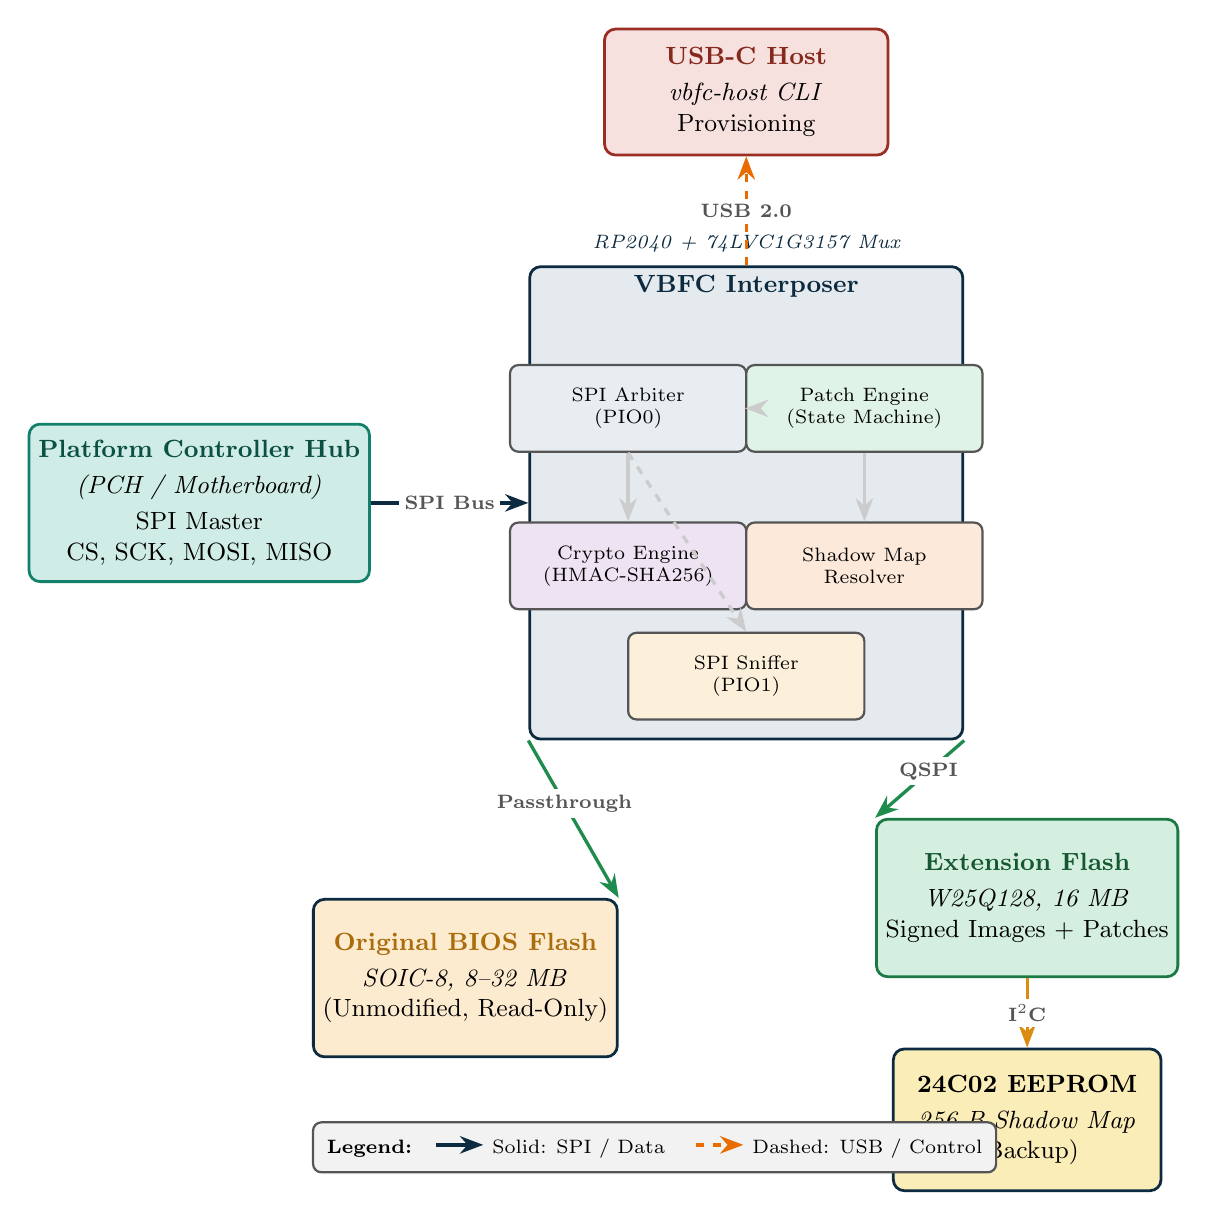
\begin{tikzpicture}[
    node distance=14mm and 20mm,
    component/.style={
        draw=vbfcDarkBlue, line width=1pt, rounded corners=4pt,
        fill=vbfcBlue!15, minimum height=20mm, minimum width=40mm,
        align=center, font=\small
    },
    storage/.style={
        draw=vbfcDarkBlue, line width=1pt, rounded corners=4pt,
        fill=vbfcOrange!20, minimum height=20mm, minimum width=38mm,
        align=center, font=\small
    },
    ee/.style={
        draw=vbfcDarkBlue, line width=1pt, rounded corners=4pt,
        fill=vbfcYellow!30, minimum height=18mm, minimum width=34mm,
        align=center, font=\small
    },
    subcomp/.style={
        draw=vbfcDarkGray, line width=0.8pt, rounded corners=3pt,
        fill=white, minimum height=11mm, minimum width=30mm,
        align=center, font=\scriptsize
    },
    arrow/.style={-Stealth, line width=1.2pt, draw=vbfcDarkBlue},
    dasharrow/.style={-Stealth, line width=1.2pt, draw=vbfcAccent, dashed},
    greenarrow/.style={-Stealth, line width=1.2pt, draw=vbfcGreen!80!black},
    orangearrow/.style={-Stealth, line width=1.2pt, draw=vbfcOrange!90!black},
    labelstyle/.style={font=\scriptsize\bfseries, text=vbfcDarkGray, fill=white, inner sep=2pt},
]

% PCH (Motherboard)
\node[component, fill=vbfcTeal!20, draw=vbfcTeal!80!black] (pch) {
    \textbf{\color{vbfcTeal!50!black}Platform Controller Hub}\\[2pt]
    \textit{(PCH / Motherboard)}\\[2pt]
    SPI Master \\ \small CS, SCK, MOSI, MISO
};

% VBFC Interposer (big box)
\node[component, fill=vbfcBlue!12, minimum width=55mm, minimum height=60mm, anchor=west] (vbfc) at ($(pch.east)+(20mm,0)$) {};
\node[font=\small\bfseries, text=vbfcDarkBlue, anchor=north] at (vbfc.north) {VBFC Interposer};
\node[font=\scriptsize\itshape, text=vbfcDarkGray, anchor=north] at ($(vbfc.north)+(0,5mm)$) {\color{vbfcDarkBlue}RP2040 + 74LVC1G3157 Mux};

% Sub-components inside VBFC
\node[subcomp, fill=vbfcBlue!10] (arbiter)    at ($(vbfc.center)+(-15mm,12mm)$) {SPI Arbiter\\(PIO0)};
\node[subcomp, fill=vbfcGreen!15] (patch)     at ($(vbfc.center)+(15mm,12mm)$) {Patch Engine\\(State Machine)};
\node[subcomp, fill=vbfcPurple!15] (crypto)   at ($(vbfc.center)+(-15mm,-8mm)$) {Crypto Engine\\(HMAC-SHA256)};
\node[subcomp, fill=vbfcAccent!15] (shadow)   at ($(vbfc.center)+(15mm,-8mm)$) {Shadow Map\\Resolver};
\node[subcomp, fill=vbfcOrange!15] (sniffer)  at ($(vbfc.center)+(0mm,-22mm)$) {SPI Sniffer\\(PIO1)};

\draw[arrow, draw=vbfcMediumGray] (arbiter.east) -- (patch.west);
\draw[arrow, draw=vbfcMediumGray] (arbiter.south) -- (crypto.north);
\draw[arrow, draw=vbfcMediumGray] (patch.south) -- (shadow.north);
\draw[arrow, draw=vbfcMediumGray, dashed] (arbiter.south) -- (sniffer.north);

% USB interface
\node[component, fill=vbfcRed!15, draw=vbfcRed!80!black, minimum height=16mm, minimum width=36mm] (usb) at ($(vbfc.north)+(0mm,22mm)$) {
    \textbf{\color{vbfcRed!70!black}USB-C Host}\\[2pt]
    \textit{vbfc-host CLI}\\ Provisioning
};

% Original flash
\node[storage, anchor=north] (orig_flash) at ($(vbfc.south west)+(-8mm,-20mm)$) {
    \textbf{\color{vbfcOrange!70!black}Original BIOS Flash}\\[2pt]
    \textit{SOIC-8, 8--32 MB} \\ (Unmodified, Read-Only)
};

% Extension flash
\node[storage, fill=vbfcGreen!20, draw=vbfcGreen!70!black] (ext_flash) at ($(vbfc.south east)+(8mm,-20mm)$) {
    \textbf{\color{vbfcGreen!50!black}Extension Flash}\\[2pt]
    \textit{W25Q128, 16 MB} \\ Signed Images + Patches
};

% EEPROM
\node[ee] (eeprom) at ($(ext_flash.south)+(0mm,-18mm)$) {
    \textbf{24C02 EEPROM}\\[2pt]
    \textit{256 B Shadow Map} \\ (Backup)
};

% Arrows
\draw[arrow] (pch.east) -- node[labelstyle] {SPI Bus} (vbfc.west);
\draw[greenarrow] (vbfc.south west) -- node[labelstyle, pos=0.4] {Passthrough} (orig_flash.north east);
\draw[greenarrow] (vbfc.south east) -- node[labelstyle, pos=0.4] {QSPI} (ext_flash.north west);
\draw[dasharrow] (vbfc.north) -- node[labelstyle, pos=0.5] {USB 2.0} (usb.south);
\draw[orangearrow] (ext_flash.south) -- node[labelstyle, pos=0.5] {I$^2$C} (eeprom.north);

% Legend
\node[draw=vbfcDarkGray, line width=0.8pt, rounded corners=3pt, fill=vbfcLightGray,
      anchor=north west, font=\scriptsize, inner sep=5pt] at ($(orig_flash.south west)+(0mm,-8mm)$) {
    \textbf{Legend:}\quad
    \tikz\draw[arrow] (0,0) -- (6mm,0);~Solid: SPI / Data \quad
    \tikz\draw[dasharrow] (0,0) -- (6mm,0);~Dashed: USB / Control
};

\end{tikzpicture}
\end{document}
